\documentclass{article}
\usepackage{graphicx} % Required for inserting images
\usepackage{amsmath, amssymb}
\usepackage{hyperref}
\title{Parallel t-SVDM: A Multi-Backend Performance Study \\
       \large CS 2050 Final Project}
\author{Luca Grossmann}
\date{May 2026}

\begin{document}

\maketitle

\section{Introduction}

Much of modern data is multilinear by nature. A video might be stored in a
tensor with ``height,'' ``width,'' and ``frames'' dimensions; a multi-omics
dataset stacks measurements across patients, variables, and time points.
Tensors, which are multi-way arrays, have become a natural way to store these
higher-dimensional datasets. Despite this, the tendency is still to
``flatten'' or ``matricize'' the data before analyzing or compressing it.
Flattening allows for the use of powerful traditional linear-algebraic tools
such as PCA and SVD, but it ignores higher-dimensional correlations that
might be stored in the data. Recently there have been advances in
low-order tensor decomposition methods, with modern algorithms such as the
t-SVDM, introduced in \cite{kilmer2021tensor}, achieving Eckart--Young-like
optimality guarantees that older tensor methods cannot match.

From a high-performance-computing standpoint, the t-SVDM is a particularly
appealing target. Its dominant cost is a sequence of $n$ matrix singular
value decompositions, one per frontal slice of the transformed tensor, which
are completely independent of one another. The surrounding forward and inverse
transforms each reduce to a single dense matrix--matrix multiplication. The
algorithm is therefore embarrassingly parallel at the slice level, where most of the work is being done. 

In this report we present and benchmark five implementations of the full
t-SVDM: a serial C++ baseline using LAPACK, an OpenMP version that
parallelizes the slice loop, an MPI version that distributes slices across
ranks, a GPU version using CuPy, and an additional Julia implementation
written in the standard library. All five are validated by reconstruction
error (Section~\ref{subsec:correctness}) and cross-checked against the
Python reference, which is itself oracle-tested against the canonical
Python implementation \texttt{mprod\_package}~\cite{kilmer2021tensor}.
The remainder of the report introduces the algorithm formally
(Section~\ref{subsec:tsvdm}), describes each implementation
(Section~\ref{sec:methods}), and reports strong-scaling, weak-scaling, and
profiling results (Section~\ref{sec:results}).
\subsection{The t-SVDM}
\label{subsec:tsvdm}
Let $A \in \mathbb{R}^{m \times p \times n}$ be a third-order tensor, which we
will think of as subjects $\times$ variables $\times$ time, though this
labeling is inconsequential to the underlying math. Following MATLAB-style
indexing, $A_{:,:,i}$ denotes the $i$-th \emph{frontal slice} and $A_{i,j,:}$ a
\emph{tube fiber} (Figure~\ref{fig:tensor}).
We use the tensor Frobenius norm $\Vert A \Vert_F^2 =
\sum_{i,j,k} \vert A_{i,j,k} \vert^2$ \cite{Kolda2009}.
\begin{figure}[h]
    \centering
    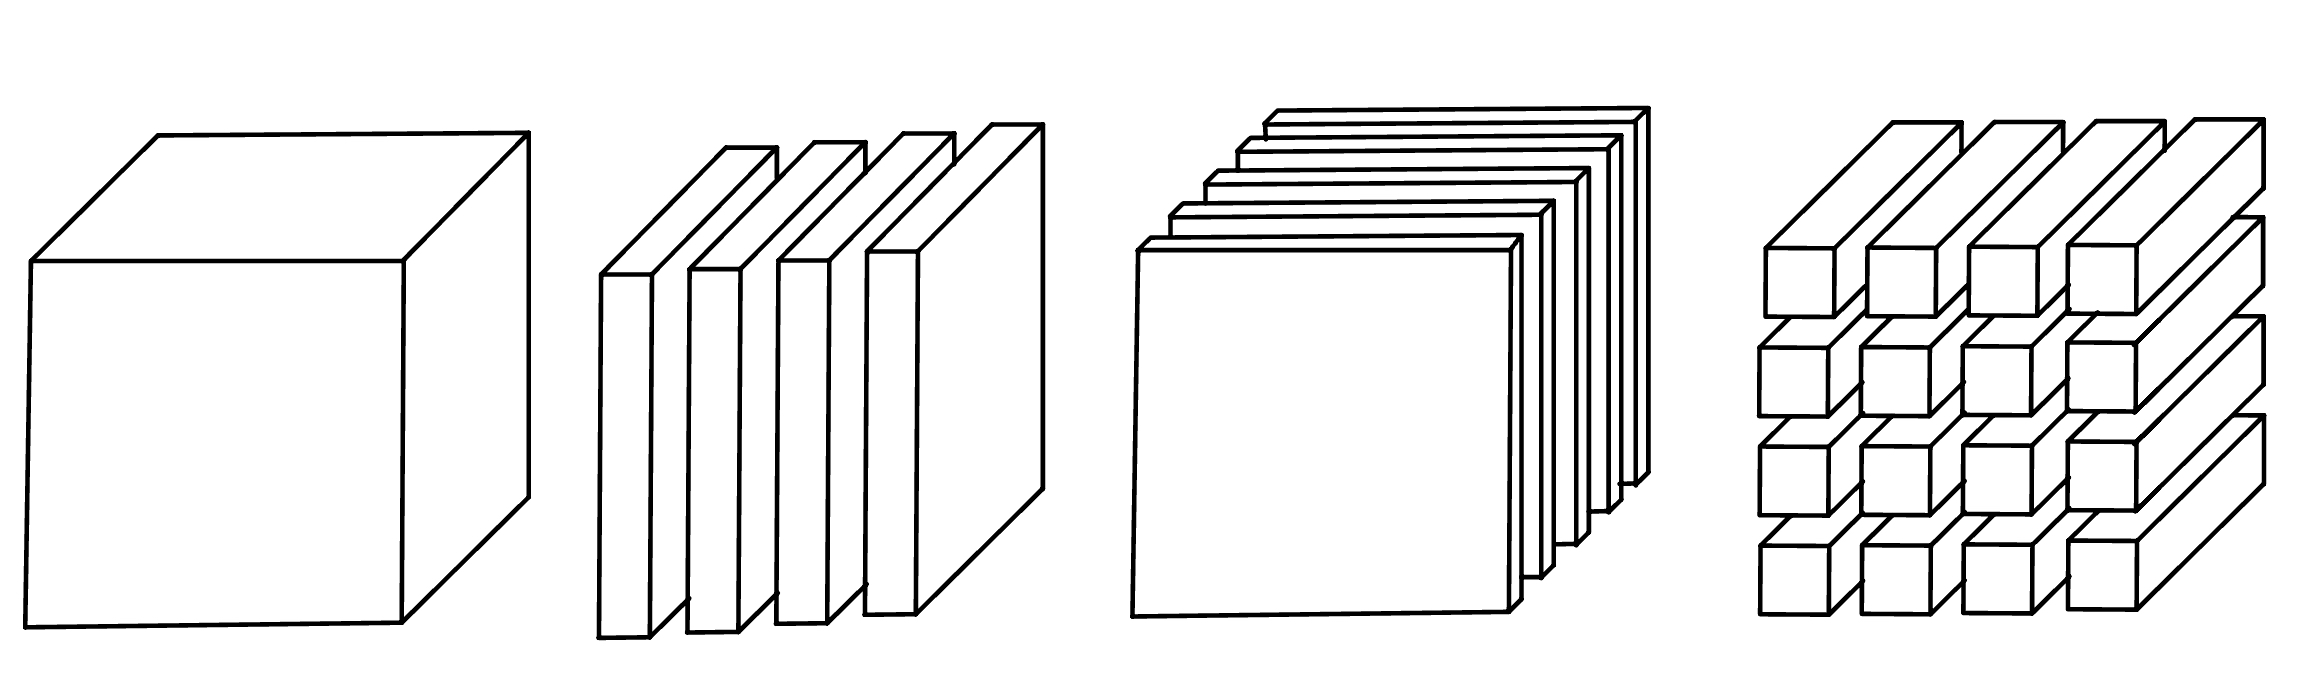
\includegraphics[width=0.8\textwidth]{figures/tensor.jpg}
    \caption{Left to Right: Tensor $X$, Lateral Slices $X_{:,j,:}$, Frontal Slice  $A_{:,:,i}$, Tube Fiber $A_{i,j,:}$}
    \label{fig:tensor}
\end{figure}

\paragraph{Mode-3 product.} For an $n \times n$ matrix $\textbf{B}$, the mode-3
tensor-matrix product $A \times_3 \textbf{B}$ is defined via the mode-3
unfolding $\textbf{A}_{(3)} \in \mathbb{R}^{n \times mp}$, whose columns are
the tube fibers of $A$: we compute $\textbf{B}\,\textbf{A}_{(3)}$ and fold the
result back into a tensor of the same shape \cite{Kolda2009}. Equivalently,
for each tube fiber we apply the matrix-vector product $\textbf{B}\,A_{i,j,:}$ (Figure~\ref{fig:Mode3}).
When $\textbf{B}$ is orthogonal, this rotates each tube fiber into a transform
domain in which $A$ is more compressible.

\begin{figure}
    \centering
    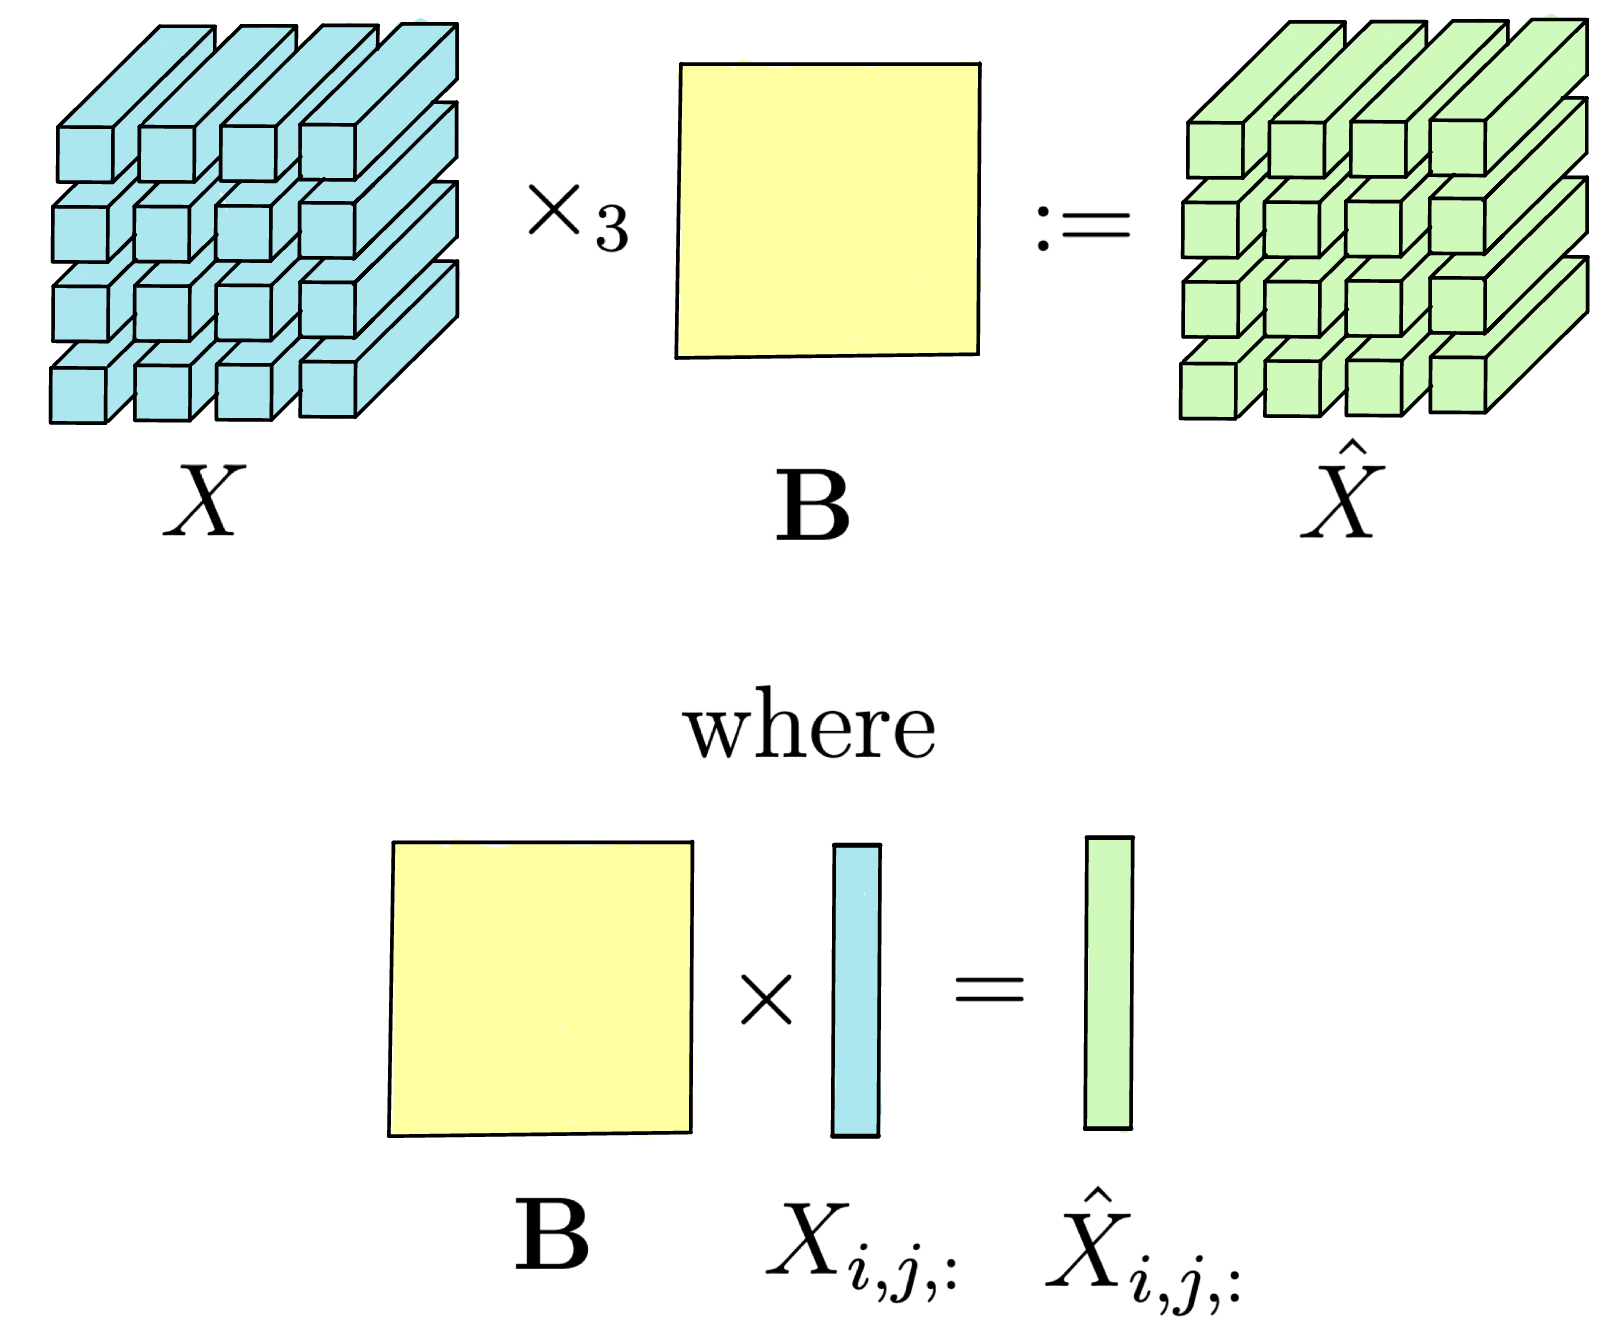
\includegraphics[width=0.6\linewidth]{figures/mode_3_prod.jpg}
    \caption{Mode 3 Product}
    \label{fig:Mode3}
\end{figure}
\paragraph{The $\star_\textbf{M}$ product.} For invertible $\textbf{M} \in
\mathbb{R}^{n \times n}$, write $\hat{A} := A \times_3 \textbf{M}$ for the
transform-domain representation. The $\star_\textbf{M}$ tensor-tensor product,
introduced in \cite{tprod} and generalised in \cite{kilmer2021tensor}, is
defined for $A \in \mathbb{R}^{m \times p \times n}$ and
$B \in \mathbb{R}^{p \times l \times n}$ by:
\begin{enumerate}
    \item $\hat{A} \leftarrow A \times_3 \textbf{M}$,\quad $\hat{B} \leftarrow B \times_3 \textbf{M}$;
    \item for $i = 1, \dots, n$:\quad $\hat{C}_{:,:,i} = \hat{A}_{:,:,i}\, \hat{B}_{:,:,i}$;
    \item $C = \hat{C} \times_3 \textbf{M}^{-1}$.
\end{enumerate}
The face-wise multiplications in step~2 are independent across $i$, so the
$\star_\textbf{M}$ product is naturally parallel.

\paragraph{Definition (t-SVDM \cite{kilmer2021tensor}).} The full
$\star_\textbf{M}$ tensor SVD of $A \in \mathbb{R}^{m \times p \times n}$ is
\[
A \;=\; U \star_\textbf{M} S \star_\textbf{M} V^H,
\]
where $U \in \mathbb{R}^{m \times m \times n}$ and $V \in \mathbb{R}^{p \times
p \times n}$ are $\star_\textbf{M}$-unitary, and $S \in \mathbb{R}^{m \times p
\times n}$ has diagonal frontal slices. When $\textbf{M} = c\textbf{W}$ for
unitary $\textbf{W}$ and $c \neq 0$, this decomposition admits an
Eckart--Young-like optimality result: the $t$-rank-$k$ truncation of the
t-SVDM is the best $\star_\textbf{M}$ rank-$k$ approximation of $A$ in
Frobenius norm \cite{kilmer2021tensor}.

\paragraph{Algorithm (Full t-SVDM).}
\begin{enumerate}
    \item $\hat{A} \leftarrow A \times_3 \textbf{M}$;
    \item for $i = 1, \dots, n$:
        $\;\bigl[\hat{U}_{:,:,i},\, \hat{S}_{:,:,i},\, \hat{V}_{:,:,i}\bigr] = \mathrm{svd}\bigl(\hat{A}_{:,:,i}\bigr)$;
    \item $U = \hat{U} \times_3 \textbf{M}^{-1}$,
          $S = \hat{S} \times_3 \textbf{M}^{-1}$,
          $V = \hat{V} \times_3 \textbf{M}^{-1}$;
    \item return $U, S, V$.
\end{enumerate}

The t-SVDM brings $A$ into the transform space by applying $\textbf{M}$,
computes and stores the SVD of every frontal slice of $\hat{A}$, then returns
to the spatial domain by applying $\times_3 \textbf{M}^{-1}$ to each output (Figure~\ref{fig:tSVDM_diagram}).
The motivation is that with a smart choice of orthogonal $\textbf{M}$ ( the Discrete Fourier Transform is a common choice) $\hat{A}$ can be far
more compressible than $A$ given the rotation of each tube fiber
\cite{kilmer2021tensor}. From an HPC standpoint, step~2 dominates cost and
consists of $n$ independent matrix SVDs, while steps~1 and~3 reduce to
single dense matrix--matrix products after reshaping. This structure is
exactly what makes the t-SVDM an attractive target for parallelization.

\begin{figure}
    \centering
    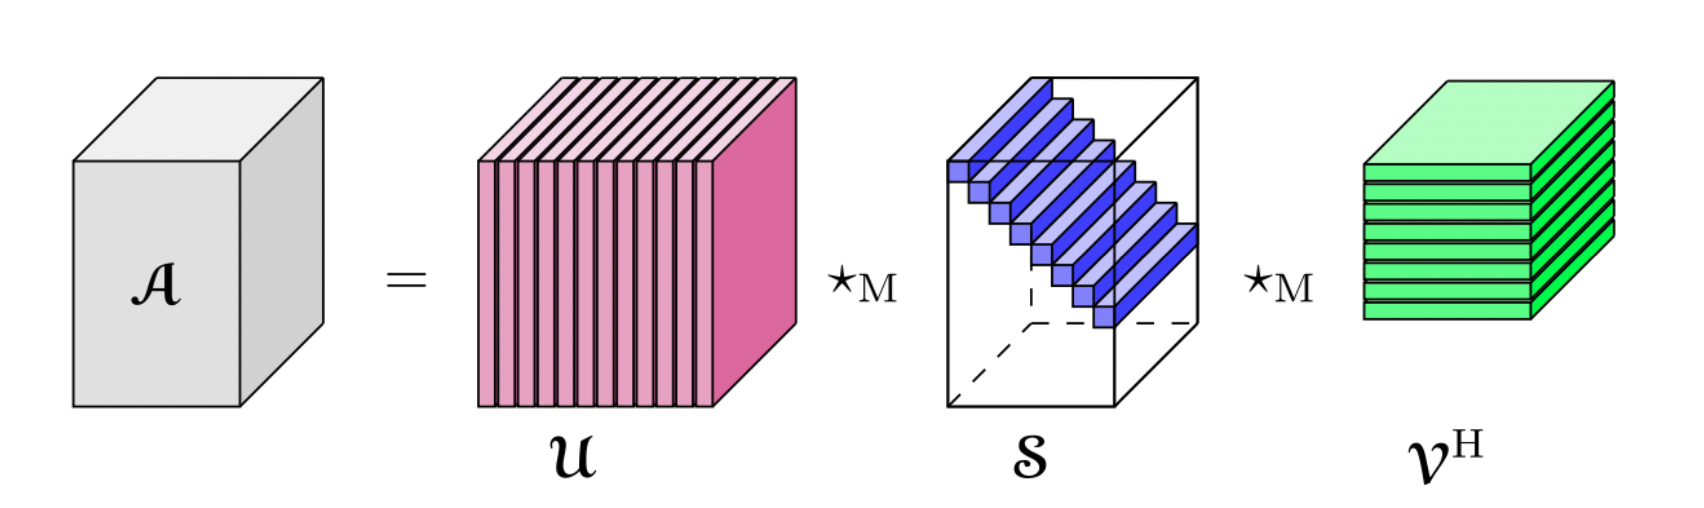
\includegraphics[width=0.9\linewidth]{figures/tSVDM_diagram.png}
    \caption{tSVDM (adapted from \cite{kilmer2021tensor})}
    \label{fig:tSVDM_diagram}
\end{figure}


\section{Methods}
\label{sec:methods}

\subsection{Serial C++ baseline}
The serial baseline is a single C++ file that calls LAPACK routines directly, 
with OpenBLAS (installed via Spack) providing the implementations. We
store $A$ column-major in shape $(m, p, n)$, so each frontal slice is a contiguous
block of size $mp$ that can be passed to LAPACK without copying.The mode-3 transform exploits the fact that this memory layout is identical to a column-major
$(mp) \times n$ matrix on a byte level, so $A \times_3 \mathbf{M}$ reduces to a single
\texttt{dgemm} call. We can compute the inverse transform by changing the 
\texttt{transb} flag. The per-slice SVDs are produced by
\texttt{dgesdd}. The shared workspace only needs to be queried once via 
\texttt{lwork = -1} as matrix dimensions are constant across slices. Finally, OpenBLAS
is fixed to one thread to isolate the baseline timing from any BLAS-level parallelism.

\subsection{OpenMP}
The OpenMP implementation parallelizes the embarrassingly parallel per-slice loops of the serial
baseline. We speed up the dominant loop, containing the $n$
independent \texttt{dgesdd} calls, through 
\texttt{\#pragma omp parallel for schedule(dynamic)}. 
SVD cost varies between each $\hat{A}_{:,:,i}$, which motivates the dynamic schedule. 
Because LAPACK scratch buffers can't be shared between threads, each thread allocates its own \texttt{work} and \texttt{iwork}, reused across all its slices.
Guided by  VTune (Section~\ref{subsec:profiling}) we used similar patterns on the 
remaining lower cost operations. 
These included the assembly of $\hat{S}$, the $\star_M$ transpose 
$\hat{V}^T$ into $\hat{V}$, and the facewise matrix multiply used in reconstruction. 
 The mode-3 \texttt{dgemm}s stay serial with
\texttt{OPENBLAS\_NUM\_THREADS=1} to avoid nested parallelism
collapsing efficiency. We sweep \texttt{OMP\_NUM\_THREADS} over
$\{1, 2, 4, 8, 16\}$ to test strong scaling (Section~\ref{subsec:strong}).



\subsection{MPI}
The MPI implementation distributes the dominant per-slice SVD loop across
ranks. Each rank owns a contiguous block of $\mathrm{count} = n / P$
slices starting at $\mathrm{start} = r \cdot \mathrm{count}$. Every rank reads the
fixture from disk independently. Each rank then runs the forward
mode-3 \texttt{dgemm} on the full tensor and calls the serial baseline's
\texttt{sliceSvdAll} helper on its assigned slices. We then use three 
\texttt{MPI\_Allgather} calls to reassemble $\hat{U}$,
$\hat{s}$, and $\hat{V}^T$ on every rank. The operations after the slice-wise SVD: building
$\hat{S}$, transposing $\hat{V}^T$ into $\hat{V}$, and the three inverse
mode-3 \texttt{dgemm}s also runs on every rank, so all inter-rank
communication is contained in a single allgather. We set 
\texttt{OPENBLAS\_NUM\_THREADS=1} to ensure that MPI is  the only source of
parallelism. We synchronize ranks with \texttt{MPI\_Barrier} before each rep, time the call with \texttt{MPI\_Wtime}, and    
aggregate the slowest rank's time with \texttt{MPI\_Reduce(MPI\_MAX)}.  Rank 0 reconstructs the tensor
and prints the result line. We sweep $P \in \{1, 2, 4, 8\}$ across
nodes for strong scaling.

\subsection{CUDA via CuPy}
The CuPy implementation expresses the full t-SVDM in a handful of GPU calls.
A small \texttt{mode3(X, A)} helper handles both the forward and inverse
mode-3 transforms as a \texttt{reshape}--\texttt{matmul}--\texttt{reshape},
mirroring the serial \texttt{dgemm} trick: the $(n, m, p)$ tensor and the
$(n, mp)$ matrix occupy identical memory, so each mode-3 product becomes a
single cuBLAS \texttt{dgemm}. The dominant per-slice SVDs collapse into one
batched call, \texttt{cp.linalg.svd(A\_hat, full\_matrices=False)}, which
dispatches internally to a cuSOLVER routine. The f-diagonal $\hat{S}$ is built by
fancy-indexed assignment, and the three inverse mode-3 transforms reuse
\texttt{mode3} with $M^T$. We bracket the timed region with
\texttt{cp.cuda.Stream.null.synchronize()} so kernel-launch asynchrony does
not bleed into the wall-clock measurement. The cluster's GPU pool is heterogeneous (L4 or
A10G are scheduled depending on availability); both are inference-class,
with FP64 (standard in numerical linear algebra)throughput in the 0.5--1.0\,TFLOPS range. The production run we
report below landed on an A10G.

\subsection{Additional implementation: Julia}
We chose Julia for the additional implementation given its prominence 
in the numerical linear algebra community. The implementation uses only the standard 
library (\texttt{LinearAlgebra}, \texttt{Random}, \texttt{Printf}). A 
\texttt{mode3(X, A)} helper handles both the forward and inverse mode-3 
transforms as a single \texttt{reshape}--\texttt{matmul}--\texttt{reshape} 
that calls BLAS \texttt{dgemm}. The per-slice loop calls \texttt{svd} 
(LAPACK \texttt{dgesdd}), and the f-diagonal $\hat{S}$ is assembled via 
the stdlib \texttt{Diagonal} wrapper. We implemented only a serial 
version for direct comparison with the C++ baseline, at roughly $\sim$130 
lines versus $\sim$350 in C++. Working in Julia is often a 
simpler process, especially to those familiar with Python. 
To ensure fair timing, we include an 
untimed warmup call that amortizes Julia's first-run JIT cost.


\section{Results}
\label{sec:results}

\subsection{Correctness}
\label{subsec:correctness}
After the \texttt{tsvdm} call, every backend reconstructs the original tensor
$\tilde{A} = U \star_\mathbf{M} S \star_\mathbf{M} V^H$ and reports the
relative Frobenius error $\Vert A - \tilde{A}\Vert_F / \Vert A \Vert_F$. We compare
reconstructions rather than the factors themselves to avoid sign ambiguity which can cause comparisons to fail even when
both implementations are correct. The Python reference in \texttt{cuda/tsvdm\_core.py} is itself cross-validated
against \texttt{mprod\_package} \cite{kilmer2021tensor} via
\texttt{cuda/tests/test\_oracle.py}, which checks that both libraries reconstruct the
same input to within $10^{-10}$. Each C++/CuPy/Julia backend additionally
supports a \texttt{--dump} flag that writes its reconstruction to disk, enabling element-wise cross-checks with
\texttt{cuda/compare\_cpp\_python.py}. Across all implementations and
problem sizes, the relative error sits near FP64 round-off$(\sim 10^{-15})$. 


\subsection{Strong scaling}
\label{subsec:strong}
We hold the problem size fixed and sweep the number of workers. Two
fixtures bracket the regime: \emph{medium} ($m=p=n=256$,
$\sim 128$\,MB) sits comfortably in cache, while \emph{large}
($m=p=512$, $n=256$, $\sim 512$\,MB) exceeds it. Strong-scaling
results for OpenMP and MPI on both fixtures appear in
Figure~\ref{fig:strong}, and the corresponding parallel efficiencies
at the medium fixture are summarised in
Figure~\ref{fig:eff_bars}.

\begin{figure}[h]
    \centering
    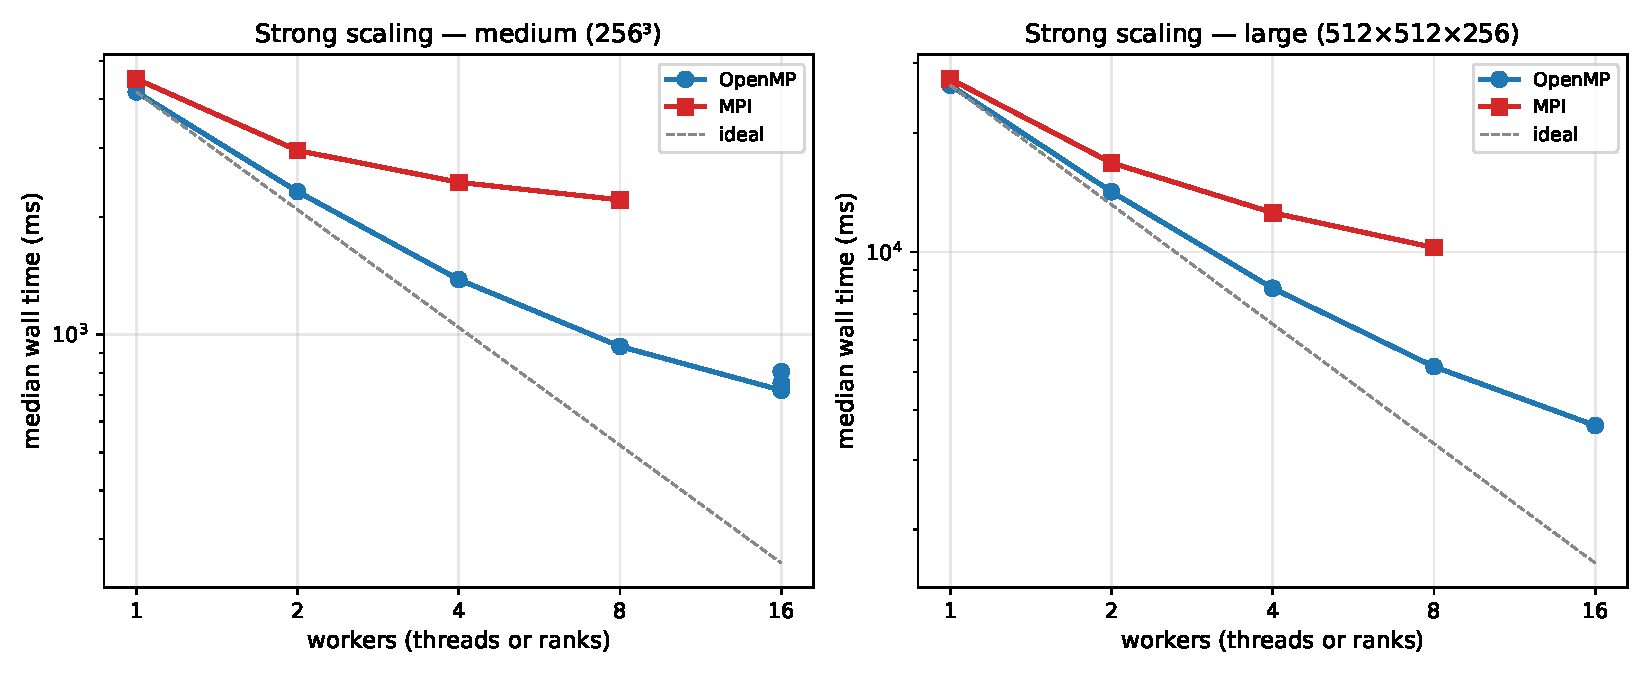
\includegraphics[width=\linewidth]{figures/strong_scaling.pdf}
    \caption{Strong scaling of OpenMP (blue circles) and MPI (red squares) on the medium ($256^{3}$, left) and large ($512{\times}512{\times}256$, right) fixtures. Dashed line is ideal speedup relative to the single-worker baseline.}
    \label{fig:strong}
\end{figure}

\begin{figure}[h]
    \centering
    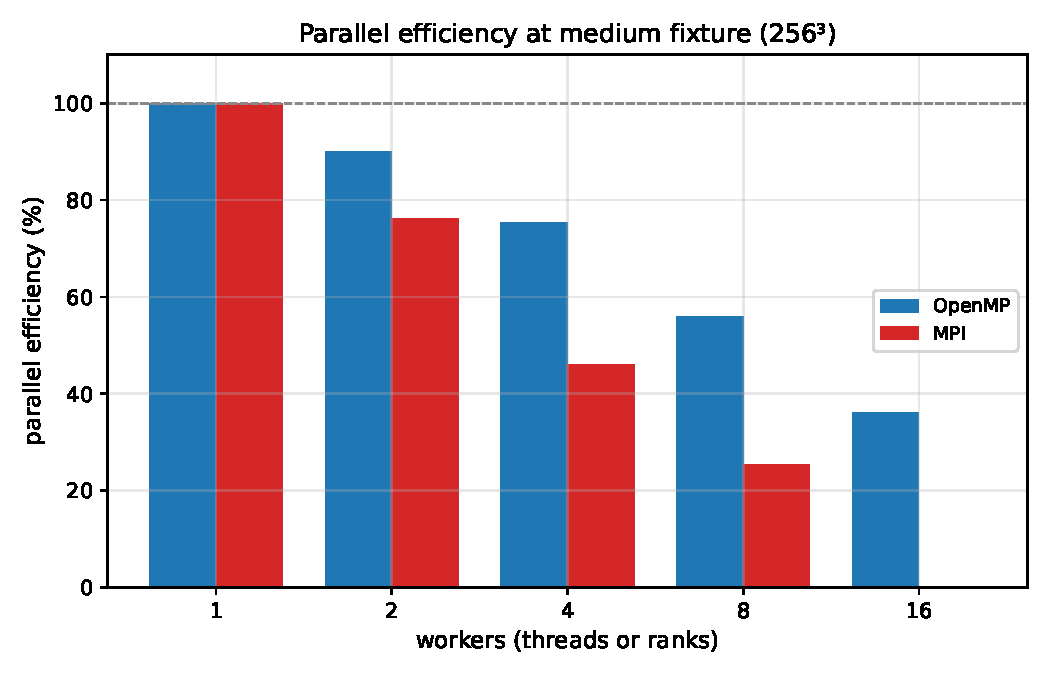
\includegraphics[width=0.85\linewidth]{figures/efficiency_bars.pdf}
    \caption{Parallel efficiency at the medium fixture. OpenMP retains $36\%$ efficiency at $T=16$, while MPI collapses to $25\%$ at $P=8$.}
    \label{fig:eff_bars}
\end{figure}

\paragraph{OpenMP.} On the medium fixture, runtime falls from
$4173$\,ms at $T=1$ to $721$\,ms at $T=16$, a $5.79\times$ speedup
($36\%$ efficiency). The large fixture scales noticeably better
($26{,}344$\,ms $\to$ $3{,}657$\,ms, a $7.20\times$ speedup at $45\%$
efficiency) because the per-thread SVD work dominates the constant
serial cost of the two mode-3 \texttt{dgemm}s, which we keep
single-threaded to avoid nested parallelism. The remaining gap from
ideal is a textbook Amdahl floor: the two single-threaded \texttt{dgemm}s
plus OpenMP fork-join overhead form a fixed serial component that
caps speedup, especially on the smaller medium fixture where SVD
work is shorter.

\paragraph{MPI.} MPI's strong scaling is much weaker than OpenMP's:
medium goes $4504\,\text{ms} \to 2211$\,ms across $P\in\{1,2,4,8\}$,
a mere $2.04\times$ speedup ($25\%$ efficiency at $P=8$). The large
fixture does better ($27{,}313 \to 10{,}268$\,ms, $2.66\times$,
$33\%$) but still trails OpenMP. Two structural choices explain it:
every rank performs the full forward and inverse mode-3
\texttt{dgemm}s redundantly, and the three \texttt{MPI\_Allgather}
calls that reassemble $\hat{U}$, $\hat{s}$, $\hat{V}^{T}$ have
fixed-size payloads independent of $P$, so per-rank network cost stays
constant while per-rank compute shrinks. The result is an efficiency
curve that decays faster than Amdahl alone would predict; the gap
between OpenMP and MPI in Figure~\ref{fig:eff_bars} reflects that
extra communication-bound term.

\subsection{Weak scaling}
\label{subsec:weak}
Weak scaling holds per-worker work constant by growing the problem
with the worker count. We fix slice geometry at $m=p=256$ and scale
the number of frontal slices $n = 32 \cdot W$, where $W$ is the
number of threads (OpenMP) or ranks (MPI). Ideal weak scaling
appears as a flat runtime curve.

\begin{figure}[h]
    \centering
    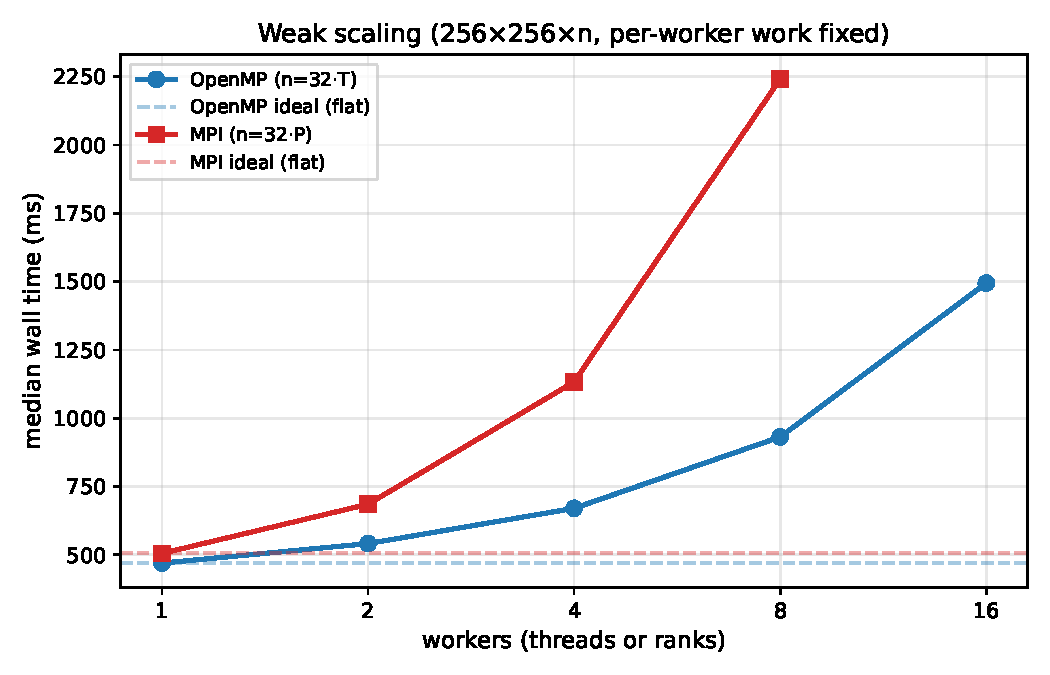
\includegraphics[width=0.75\linewidth]{figures/weak_scaling.pdf}
    \caption{Weak scaling at $256\times 256 \times (32\,W)$. Dashed lines mark each backend's single-worker runtime, the flat ideal. OpenMP holds reasonable efficiency through $T=4$; MPI degrades immediately.}
    \label{fig:weak}
\end{figure}

OpenMP's weak-scaling efficiency is $100\%, 87\%, 70\%, 50\%, 31\%$
at $T \in \{1,2,4,8,16\}$ (runtimes $470, 541, 670, 931, 1494$\,ms).
The drop is consistent with the same Amdahl floor seen in strong
scaling: as we grow $n$ in step with $T$, the two single-threaded
mode-3 \texttt{dgemm}s grow linearly with $n$ while the parallel SVD
loop's per-thread cost stays flat; the serial contribution therefore
consumes an increasing share of total runtime.

MPI's weak-scaling drop is sharper still: $100\%, 74\%, 45\%, 23\%$
at $P \in \{1,2,4,8\}$ ($505, 685, 1133, 2241$\,ms). Two effects
compound. First, the forward and inverse mode-3 \texttt{dgemm}s are
performed redundantly on every rank, so growing $n$ inflates
per-rank compute even though only a $1/P$ slab of the SVD work is
local. Second, the three \texttt{MPI\_Allgather} payloads grow with
$n$, so communication cost rises along with the problem size. Both
effects scale unfavorably; the result is a doubling of runtime at
each step rather than a flat curve.

\subsection{Cross-implementation comparison}
\label{subsec:cross}
Figure~\ref{fig:cross} compares all five backends at the medium
fixture, normalized to the serial C++ baseline ($T_\text{serial} =
4270$\,ms).

\begin{figure}[h]
    \centering
    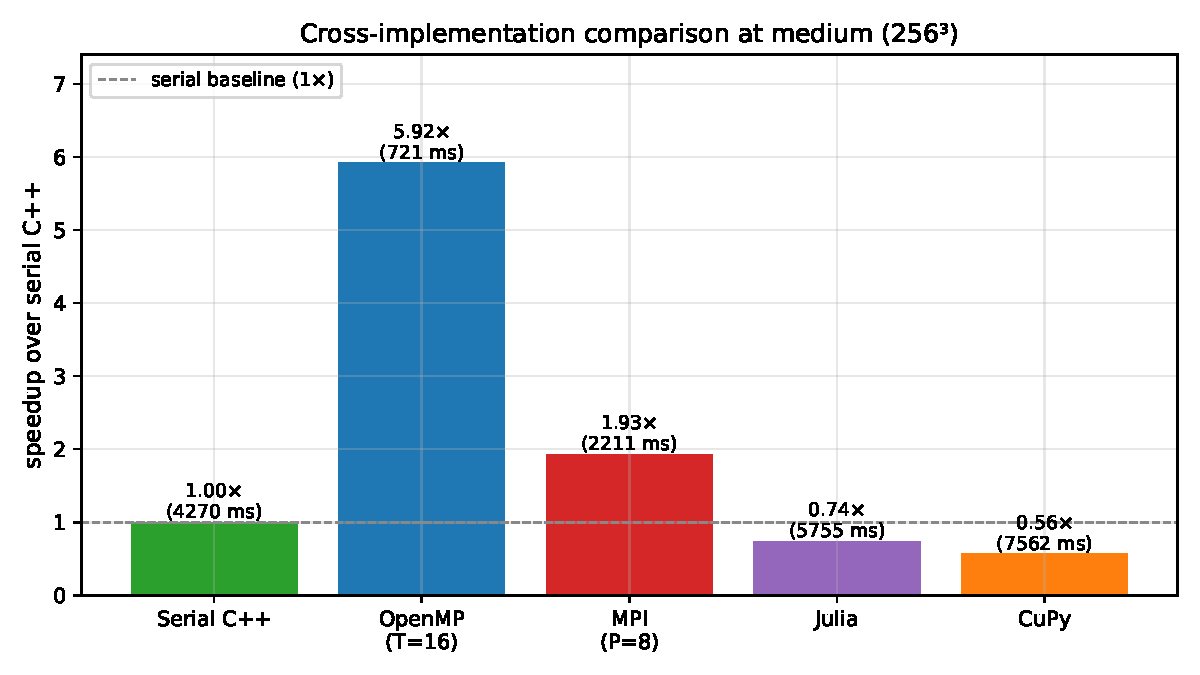
\includegraphics[width=0.85\linewidth]{figures/cross_impl_comparison.pdf}
    \caption{Speedup over serial C++ at the medium fixture (256$^3$). Heights are $T_\text{serial}/T_\text{impl}$; raw runtimes are annotated above each bar. CuPy on the A10G GPU lands below the serial CPU baseline.}
    \label{fig:cross}
\end{figure}

OpenMP at $T=16$ is the clear winner ($5.92\times$), followed by MPI
at $P=8$ ($1.93\times$); MPI's redundant per-rank GEMMs and lack of
multi-rank-per-node hybrids cost it relative to OpenMP. Julia
(stdlib) lands at $0.74\times$, slightly slower than serial C++,
consistent with calling the same LAPACK \texttt{dgesdd} through a
thicker array-machinery stack. CuPy on the A10G clocks $0.56\times$
($7562$\,ms vs.\ serial's $4270$\,ms): per-slice cuSOLVER dispatch
plus host$\leftrightarrow$device transfer push the GPU above the CPU
baseline, and the inference-class card's $\sim 1$\,TFLOPS FP64 ceiling
is roughly the same order as the 16-thread Cascade Lake node.
The same ordering holds at large size (CuPy at $22.3$\,s vs.\
OpenMP-$T{=}16$ at $3.66$\,s), so on this hardware the CPU wins
for the t-SVDM across the whole range we benchmark.

\subsection{Profiling deep-dive}
\label{subsec:profiling}
We profiled the OpenMP backend at $T=16$ on the medium fixture using
Intel VTune (Hotspots collection) in two passes, the second informed
by the first.

\paragraph{First pass --- only the SVD loop parallelized.}
The first VTune run profiles a build with \texttt{\#pragma omp
parallel for} on \texttt{sliceSvdAll} alone and the three helper
loops (\texttt{assembleSDense}, the V-slice transpose, and the
\texttt{reconstructApprox} facewise matmul) left serial. Elapsed
wall time is $4.59$\,s with a CPU time of $22.58$\,s, of which
$2.26$\,s ($10\%$) is attributed to imbalance/serial spinning.
Effective physical-core utilization sits at $18.8\%$ ($4.50$ of
$24$ available cores). The hotspot table is dominated by OpenBLAS
SKYLAKEX kernels: \texttt{dgemm\_kernel\_SKYLAKEX} ($4.43$\,s,
the mode-3 transforms), \texttt{dlasd4\_} and \texttt{dlasd3\_}
($2.56$\,s combined, the SVD kernels invoked by
\texttt{dgesdd}), and the two \texttt{dgemv\_kernel\_4x4} variants
($2.70$\,s). The per-thread timeline shows clear single thread areas
during \texttt{assembleSDense}, the V transpose, and
\texttt{reconstructApprox}: $15$ of the $16$ workers spinning while
one fills the diagonal tensor, transposes the slices, or
reconstructs. That is the reason \texttt{do\_spin} is on the hotspot
list. These three loops were the targets for a second pass,
even though each is individually cheap.

\paragraph{Second pass --- helpers parallelized.}
We added \texttt{\#pragma omp parallel for schedule(static)} to
\texttt{assembleSDense}, the V-slice transpose loop inside
\texttt{tsvdm}, and the per-slice facewise matmul loop in
\texttt{reconstructApprox}. Wall time
falls to $4.16$\,s, a $9.5\%$ reduction. The improvement is almost
entirely a reduction in OpenMP overhead: imbalance/serial-spin time
drops from $2.26$\,s to $1.37$\,s ($-39\%$); \texttt{do\_spin} from
$1.65$\,s to $1.11$\,s ($-33\%$); \texttt{blas\_memory\_alloc} from
$1.10$\,s to $0.84$\,s. Effective physical-core utilization rises only modestly,
from $18.8\%$ to $19.6\%$, because the dominant cost has not moved:
\texttt{dgemm\_kernel\_SKYLAKEX} stays at $4.41$\,s, confirming
that the first-pass pragma placement was already correct on the
algorithm's bottleneck. The second pass simply shrinks the surrounding
serial regions that previously made worker threads spin.

\paragraph{Failed BLAS-thread experiment.}
The dominant kernel \texttt{dgemm\_kernel\_SKYLAKEX} is invoked from
the four mode-3 transforms in \texttt{tsvdm}, each a single dense
$(mp) \times n$ matmul outside any OpenMP region. As a separate
experiment we tried to parallelize those calls themselves by
toggling \texttt{openblas\_set\_num\_threads(16)} at runtime around
each one, hoping OpenBLAS would distribute the matmul across the
$16$ available cores. The pass-2 trace shows the kernel time
essentially unchanged ($4.43 \to 4.41$\,s), so the runtime API did
not adjust the BLAS thread pool on this build despite our best efforts. 

\begin{figure}[h]
    \centering
    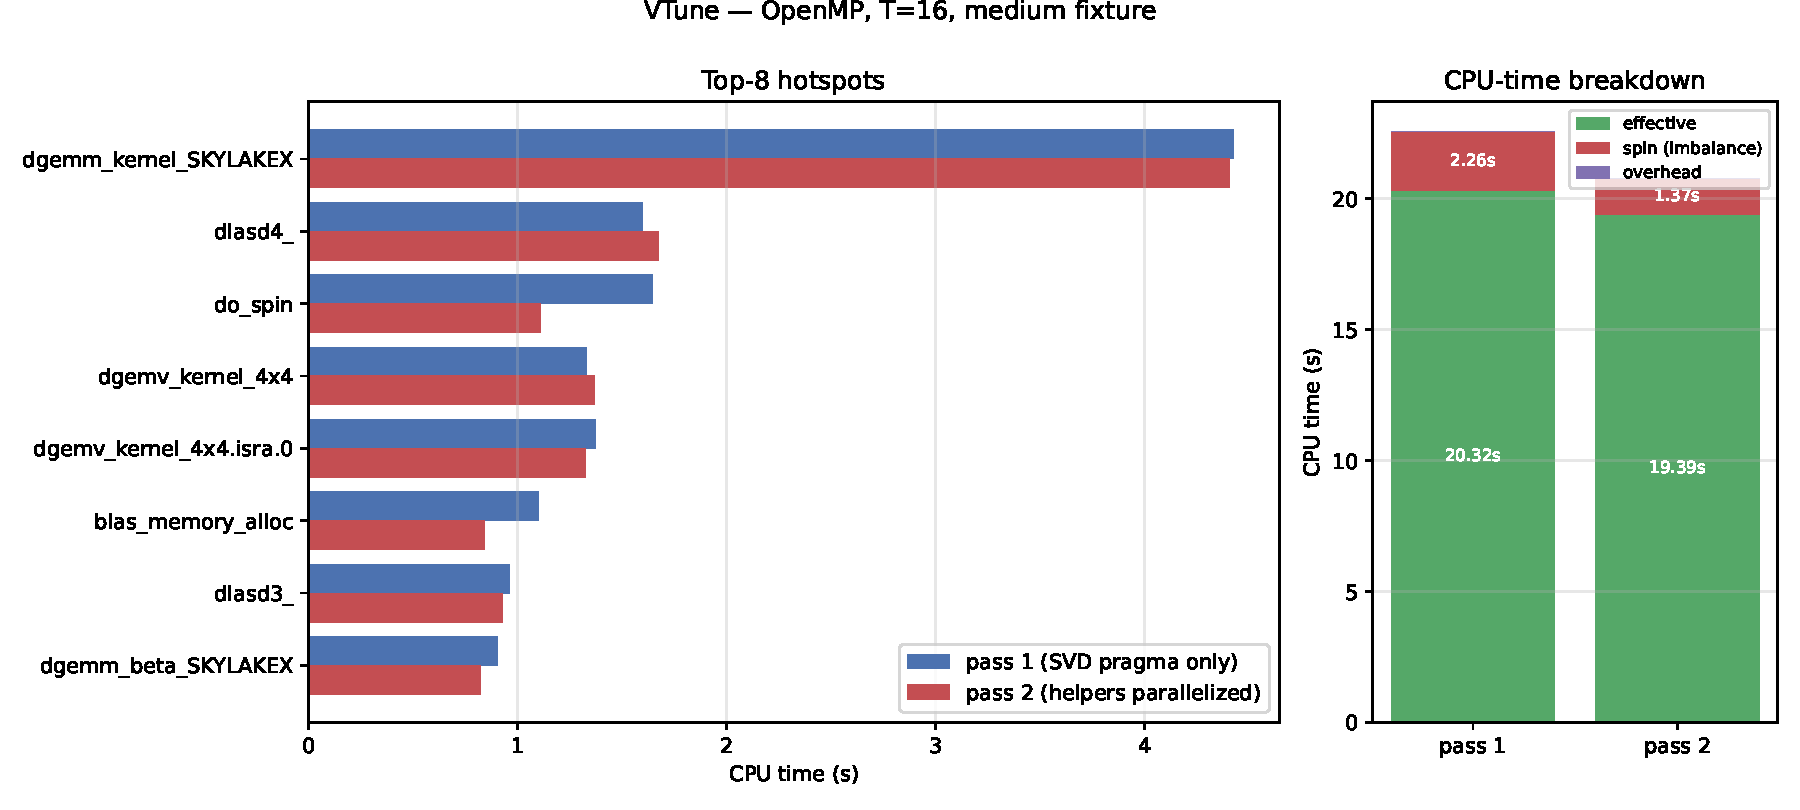
\includegraphics[width=\linewidth]{figures/profile_vtune.pdf}
    \caption{VTune profile of the OpenMP backend at $T=16$, medium fixture. Left: top-8 hotspots by CPU time, pass~1 (SVD pragma only) vs.\ pass~2 (helpers parallelized). The dominant \texttt{dgemm\_kernel\_SKYLAKEX} is essentially unchanged ($4.43 \to 4.41$\,s); the gains are in \texttt{do\_spin} ($-33\%$) and \texttt{blas\_memory\_alloc} ($-24\%$). Right: CPU-time breakdown. Spin time falls from $2.26$\,s to $1.37$\,s and effective time falls in proportion to the wall-clock improvement.}
    \label{fig:vtune}
\end{figure}

\section{Conclusion}
\label{sec:conclusion}
OpenMP at $T=16$ is the clear winner across the five backends:
$5.92\times$ on medium and $7.20\times$ on large over the serial
C++ baseline. MPI tops out at $2.04\times$ ($P=8$, medium) and
$2.66\times$ (large); weak scaling shows the cause is structural:
allgather payloads and redundant per-rank mode-3 \texttt{dgemm}s
combine into a communication-and-redundancy floor that grows with
$P$. Julia (stdlib) trails serial C++ by $\sim 1.35\times$. CuPy on
the A10G never overtakes OpenMP at any size we benchmark, despite
expressing the algorithm directly through cuBLAS and cuSOLVER. The
inference-class GPU's FP64 ceiling is the binding constraint. VTune
attributes OpenMP's remaining gap from ideal to the two
single-threaded mode-3 \texttt{dgemm}s; an attempt to engage BLAS
threads via \texttt{openblas\_set\_num\_threads} did not take effect
on the cluster's OpenBLAS build.

For dense $\star_{\mathbf{M}}$
tensor SVDs at single-node working sizes, reach for OpenMP. MPI is
worth its overhead only when the tensor exceeds a single node's
memory. GPU is not a default win on inference-class data-center
hardware; a server-class GPU or a substantially larger problem
would change that, but neither is in scope here.

\paragraph{Limitations and future work.} FP32 throughput, multi-GPU
CuPy via NCCL, hybrid OpenMP+MPI, and a rebuild of OpenBLAS with
\texttt{USE\_OPENMP=0} (so \texttt{openblas\_set\_num\_threads} would
take effect) are all out of scope. The next step is validation
on a real biological dataset: multi-omics tensors with a
biologically meaningful $\mathbf{M}$ chosen from a learned basis.

% ========================================================


\bibliographystyle{plain}
\bibliography{references}
\end{document}

